\documentclass[tikz]{standalone}

\usepackage{xcolor}
\definecolor{morange}{RGB}{255,127,14}
\definecolor{mblue}{RGB}{31,119,180}
\definecolor{mred}{RGB}{214,39,40}
\definecolor{mpurple}{RGB}{148,103,189}
\definecolor{mgreen}{RGB}{44,160,44}

\usepackage{tikz}
\usetikzlibrary{positioning}
\usetikzlibrary{calc}
\usetikzlibrary{fit}
\usetikzlibrary{shadows}
\usetikzlibrary{decorations}

\begin{document}
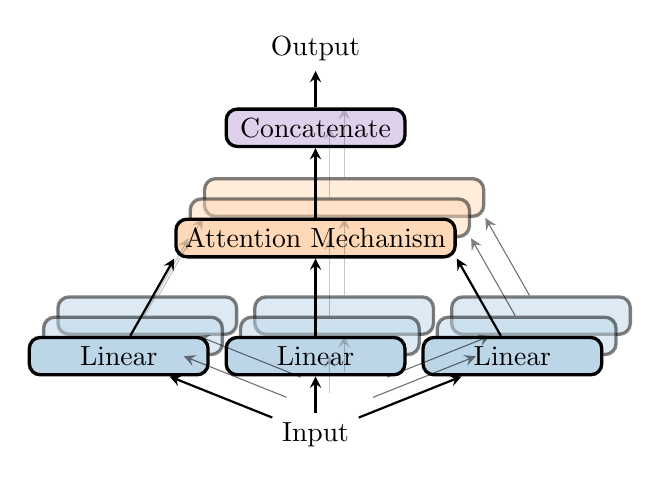
\begin{tikzpicture}[module/.style={draw, very thick, rounded corners, minimum width=15ex},
    attmodule/.style={module, fill=morange!30},
    linear/.style={module, fill=mblue!30},
    concat/.style={module, fill=mpurple!30},
    arrow/.style={-stealth, thick, rounded corners},
]
\node (input) {Input};
\node[above of=input, linear, align=center, double copy shadow={opacity=.5, shadow yshift=1.7ex, shadow xshift=1.2ex}] (linear_center) {Linear};
\node[left of=linear_center, linear, align=center, xshift=-1.5cm, double copy shadow={opacity=.5, shadow yshift=1.7ex, shadow xshift=1.2ex}] (linear_left) {Linear};
\node[right of=linear_center, linear, align=center, xshift=1.5cm, double copy shadow={opacity=.5, shadow yshift=1.7ex, shadow xshift=1.2ex}] (linear_right) {Linear};
\node[above of=linear_center, attmodule, align=center, yshift=.5cm, double copy shadow={opacity=.5, shadow yshift=1.7ex, shadow xshift=1.2ex}] (sha) {Attention Mechanism};
\node[above of=sha, concat, yshift=.4cm] (concat) {Concatenate};
\node[above of=concat] (output) {Output};

% to have the shadows displayed in the final pdf
\node[right of=linear_right, xshift=.4cm] (right_of_linear_right) {};

\draw[arrow, double copy shadow={opacity=.5, shadow yshift=1.7ex, shadow xshift=1.2ex}] (input) -- (linear_left);
\draw[arrow, double copy shadow={opacity=.2, shadow yshift=1.7ex, shadow xshift=1.2ex}] (input) -- (linear_center); 
\draw[arrow, double copy shadow={opacity=.5, shadow yshift=1.7ex, shadow xshift=1.2ex}] (input) -- (linear_right);
\draw[arrow, double copy shadow={opacity=.2, shadow yshift=1.7ex, shadow xshift=1.2ex}] (linear_left) -- (sha.south west);
\draw[arrow, double copy shadow={opacity=.2, shadow yshift=1.7ex, shadow xshift=1.2ex}] (linear_center) -- (sha.south);
\draw[arrow, double copy shadow={opacity=.5, shadow yshift=1.7ex, shadow xshift=1.2ex}] (linear_right) -- (sha.south east); 
\draw[arrow, double copy shadow={opacity=.2, shadow yshift=1.7ex, shadow xshift=1.2ex}] (sha) -- (concat.south);
\draw[arrow] (concat) -- (output);

\end{tikzpicture}
\end{document}